\chapter{UML e il diagramma delle classi}

Nel Capitolo 6 abbiamo usato il primo diagramma UML, quello dei casi d'uso, per descrivere i requisiti funzionali. In questo
capitolo vediamo che cos'è UML in generale e poi il suo diagramma più diffuso, il \textbf{diagramma delle classi}: prima la
notazione, poi il \textbf{procedimento} per costruire un modello partendo dal testo dei requisiti.

% ============================================================
\section{Modellare il dominio del problema}

\dfn{Modello di dominio}{
  Modello che descrive il \textbf{dominio del problema}. Si chiama anche \textbf{modello concettuale} o, talvolta,
  \textbf{modello di business}.
}

\warning{Problema o soluzione?}{
  Non bisogna confondere i \textbf{modelli di dominio}, che descrivono \textbf{il problema}, con i \textbf{modelli di progetto},
  che descrivono \textbf{la soluzione}. Il primo dice quali concetti esistono nel mondo reale (studenti, esami, voti); il secondo
  dice come saranno realizzati nel software (classi Java, tabelle del database, \ldots). Torneremo su questa distinzione alla fine
  del capitolo.
}

\Needspace{6\baselineskip}
Si distinguono due tipi di modelli:
\begin{itemize}
  \item i modelli \textbf{statici}, che descrivono gli \textbf{elementi} del dominio del problema e le \textbf{relazioni} tra loro;
  \item i modelli \textbf{dinamici}, che descrivono i \textbf{comportamenti} riconoscibili nel dominio del problema.
\end{itemize}

Per descrivere questi modelli si usano \textbf{linguaggi di modellazione}. In passato ogni metodologia usava i propri, nelle varie
fasi del processo di sviluppo (ad esempio i diagrammi di flusso o i \textit{Data Flow Diagram}). Negli ultimi anni si è affermato
UML come linguaggio \textbf{unificato}, usato in tutte le attività di modellazione e in molte altre attività del ciclo di vita
del software.

% ============================================================
\section{Che cos'è UML}

\dfn{UML (Unified Modelling Language)}{
  Linguaggio \textbf{grafico standard} nato per modellare software \textbf{orientato agli oggetti}. Una specifica UML definisce
  in pratica un \textbf{metamodello}: l'insieme delle regole con cui si possono costruire modelli UML.
}

\begin{figure}[H]
\centering
\begin{tikzpicture}[font=\scriptsize]
  \draw[line width=1.2pt, swgray, -{Stealth[length=3mm]}] (0,0) -- (15.6,0);
  \foreach \x/\anno/\col/\testo in {
      1.2/{fine anni '80}/swgray/{Nascono i primi processi di\\sviluppo object-oriented: tanti\\metodi e notazioni diversi},
      4.4/1994/ph4/{\textbf{Rumbaugh} e \textbf{Booch}\\uniscono i loro approcci\\alla Rational Software},
      7.4/1995/ph3/{Si unisce \textbf{Jacobson},\\che lavora sugli\\\textbf{use case}},
      10.4/1997/ph1/{L'\textbf{OMG} (Object\\Management Group) avvia\\la standardizzazione},
      13.6/2005/q8/{Prima release\\di \textbf{UML 2}}}{
    \fill[\col] (\x,0) circle (0.12);
    \node[font=\scriptsize\bfseries, text=\col, above] at (\x,0.15) {\anno};
    \node[below, align=center, text width=2.9cm] at (\x,-0.2) {\testo};
  }
\end{tikzpicture}
\caption{Le tappe principali della nascita di UML. La storia di tutte le specifiche è su \url{http://www.omg.org/spec/UML/}.}
\end{figure}

\subsection{Come si usa UML}

\begin{table}[H]
\centering
\renewcommand{\arraystretch}{1.4}
\begin{tabularx}{\textwidth}{>{\bfseries\leavevmode\color{ph4}}P{4.2cm} L}
\toprule
Uso & Descrizione \\
\midrule
Come abbozzo & Per tracciare un \textbf{modello di massima} del sistema da realizzare. \\
Come progetto & Per realizzare un \textbf{modello completo} della soluzione architetturale del sistema. \\
Come linguaggio di programmazione & Per modellare in maniera completa e precisa il sistema software. L'approccio
\textbf{MDA} (\textit{Model Driven Architecture}) esplora la possibilità di usare UML come linguaggio di programmazione.
Strumenti come \textbf{PlantUML} permettono di descrivere i diagrammi UML in forma testuale, come codice. \\
\bottomrule
\end{tabularx}
\end{table}

\subsection{Regole prescrittive e descrittive}

UML ha due tipi di regole:
\begin{itemize}
  \item le regole \textbf{prescrittive}, stabilite da organismi di standardizzazione, che fissano con precisione lessico, sintassi
        e semantica;
  \item le regole \textbf{descrittive}, che servono solo a \textbf{comunicare} il significato dei diagrammi, anche con estensioni
        libere ma intuitive delle regole di base.
\end{itemize}
Poiché lo scopo principale di UML è descrivere efficacemente situazioni reali, oggi prevalgono le regole \textbf{descrittive}.

\dfn{Regola delle informazioni soppresse}{
  L'\textbf{assenza} di un'informazione in un diagramma UML \textbf{non} significa, in generale, che quell'informazione non esista
  o sia nulla. Significa solo che è un aspetto non ancora trattato nella fase in cui il diagramma è stato tracciato, oppure che
  non lo si vuole mostrare in quel diagramma (per inserirlo in altri diagrammi).
}

\subsection{I diagrammi di UML 2}

\Needspace{12\baselineskip}
UML 2 ha \textbf{13 tipi di diagrammi}, divisi in tre categorie.

\begin{figure}[H]
\centering
\begin{tikzpicture}[font=\scriptsize]
  \node[card=q3, text width=4.6cm, align=left, minimum height=2.5cm] (c) {\textbf{\small Comportamentali}\\[3pt]
     Modellano il comportamento del sistema.\\[3pt] Es.\ casi d'uso, attività, macchine a stati.};
  \node[card=ph3, text width=4.6cm, align=left, minimum height=2.5cm, right=0.4cm of c] (i) {\textbf{\small Di interazione}\\[3pt]
     Modellano le interazioni fra le entità del sistema.\\[3pt] Es.\ \textbf{sequence diagram}, communication diagram.};
  \node[card=ph5, text width=4.6cm, align=left, minimum height=2.5cm, right=0.4cm of i] (s) {\textbf{\small Strutturali}\\[3pt]
     Modellano l'organizzazione del sistema.\\[3pt] Es.\ \textbf{class diagram}, package diagram, deployment diagram.};
\end{tikzpicture}
\caption{Le tre categorie di diagrammi di UML 2. In grassetto i due più usati.}
\end{figure}

In questo corso ci si concentra sui due diagrammi più utilizzati: il \textbf{diagramma delle classi} (questo capitolo) e il
\textbf{diagramma di sequenza} (Capitolo 8).

\info{Strumenti e riferimenti}{
  \textbf{Visual Paradigm} (\url{https://www.visual-paradigm.com/}) è un ottimo strumento per disegnare diagrammi UML, disponibile
  anche in una \textit{Community Edition} gratuita. Occasionalmente si usa anche il plug-in \textit{Diagrams} di IntelliJ IDEA
  per generare codice e diagrammi l'uno dall'altro.

  Il testo di riferimento è Martin Fowler, \textit{UML Distilled}: capitolo 1 (introduzione a UML), capitoli 3 e 5 (diagramma
  delle classi), capitolo 4 (diagramma di sequenza), capitolo 7 (diagramma dei package).
}

% ============================================================
\section{Il diagramma delle classi}

Il diagramma delle classi (\textit{class diagram}) è il più diffuso diagramma di UML. È un diagramma \textbf{statico}, che si può usare:
\begin{itemize}
  \item per la modellazione \textbf{concettuale} del dominio di un problema;
  \item per modellare le \textbf{specifiche} richieste a un sistema;
  \item per modellare l'\textbf{implementazione} (object-oriented) di un sistema software.
\end{itemize}
I suoi concetti fondamentali sono estensioni di quelli della programmazione orientata agli oggetti. Nel seguito lo presentiamo
nella versione più completa, quella usata per modellare l'implementazione.

\begin{table}[H]
\centering
\renewcommand{\arraystretch}{1.35}
\begin{tabularx}{\textwidth}{>{\bfseries\leavevmode\color{q9}}P{3.6cm} L}
\toprule
Elemento & Che cosa rappresenta \\
\midrule
Classi & I tipi di dati presenti nel sistema \\
Associazioni & I collegamenti tra istanze di classi \\
Attributi & I dati semplici presenti nelle classi e nelle loro istanze \\
Operazioni & Le funzioni svolte dalle classi e dalle loro istanze \\
Generalizzazioni & Raggruppano le classi in gerarchie di ereditarietà \\
\bottomrule
\end{tabularx}
\caption{Gli elementi principali di un diagramma delle classi.}
\end{table}

\subsection{Le classi}

Una classe si rappresenta con un \textbf{rettangolo} con il nome della classe; il concetto di classe è lo stesso della
programmazione a oggetti. Il rettangolo può avere altri due scomparti, uno per gli \textbf{attributi} e uno per le
\textbf{operazioni}, che si possono mostrare con un livello di dettaglio crescente.

\begin{center}
\begin{tikzpicture}
  \node[classe1=2.0cm] (r1) at (0,0) {Rectangle};
  \umlclass[1.9cm]{r2}{(2.6,-0.35)}{Rectangle}{}{getArea\\resize}
  \umlclass[1.9cm]{r3}{(5.2,-0.35)}{Rectangle}{height\\width}{}
  \umlclass[1.9cm]{r4}{(7.8,-0.5)}{Rectangle}{height\\width}{getArea\\resize}
  \umlclass[2.3cm]{r5}{(10.6,-0.5)}{Rectangle}{height: int\\width: int}{getArea(): int\\resize(int, int)}
  \draw[{Stealth[length=2mm]}-, swteal, line width=0.7pt] (0,-1.8) -- node[below, font=\scriptsize\itshape, text=swteal]{sempre più dettaglio (le altre informazioni sono soppresse)} (11.8,-1.8);
\end{tikzpicture}
\end{center}

\Needspace{4\baselineskip}
Tutte e cinque rappresentano la stessa classe: per la regola delle informazioni soppresse, il primo rettangolo non dice che
\texttt{Rectangle} non ha attributi, dice solo che in quel diagramma non li mostriamo. La firma completa di un'operazione è:
\begin{center}
  \texttt{\textcolor{swred}{nomeOperazione(nomeParametro: TipoParametro, \ldots): TipoRitornato}}
\end{center}

\subsection{Gli attributi}

\Needspace{14\baselineskip}
\dfn{Sintassi di un attributo}{
    \par\smallskip{\centering \texttt{\textcolor{swred}{visibilità nome molteplicità: tipo = default \{proprietà\}}}\par}\smallskip
  \begin{itemize}
    \item Il \textbf{nome} è l'unica parte obbligatoria.
    \item Il \textbf{tipo} può essere un tipo primitivo (\texttt{int}, \texttt{double}, \texttt{char}, \ldots) oppure il nome di
          una classe dello stesso diagramma (ma in quel caso, forse, andrebbe rappresentato con un'associazione).
    \item \textbf{default} è il valore iniziale dell'attributo.
    \item \textbf{\{proprietà\}} indica caratteristiche aggiuntive, ad esempio \texttt{\{readOnly\}} (sola lettura).
  \end{itemize}
}

\Needspace{10\baselineskip}
La \textbf{visibilità} ha tre livelli, che valgono sia per gli attributi sia per le operazioni:

\begin{table}[H]
\centering
\renewcommand{\arraystretch}{1.35}
\begin{tabularx}{\textwidth}{>{\centering\arraybackslash\ttfamily\bfseries}p{1.0cm} >{\bfseries}P{2.4cm} L >{\ttfamily}P{2.2cm}}
\toprule
\normalfont\textbf{Simbolo} & Visibilità & Chi può usare l'elemento & \normalfont\textbf{In Java} \\
\midrule
+ & Pubblica & Tutte le classi & public \\
\# & Protetta & Solo le classi derivate dalla classe originale & protected \\
- & Privata & Solo la classe originale & private \\
\bottomrule
\end{tabularx}
\end{table}

\Needspace{10\baselineskip}
La \textbf{molteplicità} indica \textbf{quanti} valori contiene l'attributo: così si possono rappresentare array e liste.
Il valore predefinito è \texttt{1}.

\begin{table}[H]
\centering
\renewcommand{\arraystretch}{1.3}
\begin{tabularx}{\textwidth}{>{\centering\arraybackslash\ttfamily\bfseries}p{1.6cm} L}
\toprule
\normalfont\textbf{Molteplicità} & Significato \\
\midrule
1 & Uno e uno solo (predefinita) \\
0..1 & Al più uno \\
* & Un numero imprecisato, eventualmente nessuno (equivale a \texttt{0..*}) \\
1..* & Almeno uno \\
\bottomrule
\end{tabularx}
\end{table}

Gli elementi di una molteplicità sono considerati un \textbf{insieme}: se sono ordinati si aggiunge \texttt{\{ordered\}}, se possono
esserci duplicati si aggiunge \texttt{\{nonunique\}}.

\begin{esempio}{Un attributo completo}
\begin{center}
  \texttt{\textcolor{ph4}{-} \textcolor{q8}{name} \textcolor{q5}{[1]}: \textcolor{ph3}{String} = \textcolor{swred}{"Untitled"} \{readOnly\}}
\end{center}
Un attributo \textbf{privato} di nome \texttt{name}, con un solo valore, di tipo \texttt{String}, che vale inizialmente
\texttt{"Untitled"} e non può essere modificato.
\end{esempio}

\subsection{Le operazioni}

\dfn{Sintassi di un'operazione}{
    \par\smallskip{\centering \texttt{\textcolor{swred}{visibilità nome (lista parametri): tipo-ritornato \{proprietà\}}}\par}\smallskip
  Visibilità e nome seguono le stesse regole degli attributi. Ogni parametro della lista ha la forma
  \par\smallskip{\centering \texttt{\textcolor{swred}{direzione nome: tipo = valore-di-default}}\par}\smallskip
  dove la \textbf{direzione} è \texttt{in} (input, il valore predefinito), \texttt{out} (output) o \texttt{inout} (entrambi).
  Il \textbf{tipo ritornato} dovrebbe essere un tipo appartenente a una classe standard.
}

\begin{esempio}{Dalla classe UML al codice Java}
\noindent\begin{minipage}[c]{0.38\textwidth}
\centering
\begin{tikzpicture}
  \umlclass[4.4cm]{cc}{(0,0)}{Account}{- owner: String\\- balance: double = 0\\\# history: Entry [*] \{ordered\}}{+ deposit(amount: double)\\+ balanceOn(date: Date): Money}
\end{tikzpicture}
\end{minipage}\hfill
\begin{minipage}[c]{0.58\textwidth}
\begin{lstlisting}[language=Java]
public class Account {
    private String owner;
    private double balance = 0;
    protected List<Entry> history;  // [*] {ordered}

    public void deposit(double amount) { ... }
    public Money balanceOn(Date date) { ... }
}
\end{lstlisting}
\end{minipage}

\medskip
Ogni simbolo di visibilità diventa il modificatore Java corrispondente, e un attributo con molteplicità \texttt{[*]} diventa una
collezione; \texttt{\{ordered\}} suggerisce una \texttt{List} invece di un \texttt{Set}.
\end{esempio}

% ============================================================
\section{Le associazioni}

\dfn{Associazione}{
  Un'\textbf{associazione} rappresenta una relazione (fisica o concettuale) tra classi. Si disegna come una \textbf{linea} tra le
  due classi, con un \textbf{nome}; un piccolo triangolo accanto al nome indica il \textbf{verso di lettura}.
}

\begin{center}
\begin{tikzpicture}
  \node[classe1] (p) at (0,0) {Persona};
  \node[classe1] (a) at (5,0) {Automobile};
  \draw[line width=0.7pt] (p) -- node[above, font=\scriptsize]{Possiede $\blacktriangleright$} (a);
\end{tikzpicture}
\end{center}

\Needspace{12\baselineskip}
Il triangolo dice che l'associazione si legge «la \textbf{Persona} possiede l'\textbf{Automobile}», e non «l'Automobile possiede
la Persona». Una possibile implementazione:

\begin{lstlisting}[language=Java]
class Persona {
    Automobile automobilePosseduta;
}
class Automobile {
}
\end{lstlisting}

\Needspace{16\baselineskip}
In alternativa al nome si può indicare il \textbf{ruolo} che una delle due classi ha nell'associazione, scritto vicino al suo estremo.

\noindent\begin{minipage}[c]{0.48\textwidth}
\centering
\begin{tikzpicture}
  \node[classe1] (p) at (0,0) {Persona};
  \node[classe1] (a) at (4.6,0) {Automobile};
  \draw[line width=0.7pt] (p) -- (a); \node[molt, anchor=south west] at ($(p.east)+(0.05,0.02)$) {+proprietario};
\end{tikzpicture}
\end{minipage}\hfill
\begin{minipage}[c]{0.48\textwidth}
\begin{lstlisting}[language=Java]
class Persona {
}
class Automobile {
    Persona proprietario;
}
\end{lstlisting}
\end{minipage}

\medskip
Qui la Persona ha il ruolo di \textbf{proprietario} dell'Automobile: il nome del ruolo diventa il nome dell'attributo.

\subsection{Il verso di navigazione}

\dfn{Verso di navigazione}{
  Indica in quale direzione è possibile \textbf{reperire le informazioni}: da quale classe si può arrivare all'altra.
  Si disegna con una \textbf{freccia} sulla linea dell'associazione. È un'informazione utile soprattutto nel progetto di dettaglio:
  essendo una scelta di progetto, di solito \textbf{non} compare nei diagrammi concettuali.
}

\begin{center}
\begin{tikzpicture}
  \node[classe1] (p) at (0,0) {Persona};
  \node[classe1] (a) at (5,0) {Automobile};
  \draw[navig] (p) -- node[above, font=\scriptsize]{Possiede $\blacktriangleright$} (a);
\end{tikzpicture}
\end{center}

\Needspace{8\baselineskip}
\begin{itemize}
  \item Nota una persona, è possibile sapere quali automobili possiede (se ne possiede).
  \item Nota un'automobile, \textbf{non} è possibile risalire al suo possessore.
  \item Il diagramma non dice nulla, invece, su \textbf{quante} automobili ha una persona né su quanti proprietari ha
        un'automobile: non sappiamo se sono informazioni non note o semplicemente soppresse.
\end{itemize}

\begin{esempio}{Implementazione corretta ed errata}
\noindent\begin{minipage}[t]{0.48\textwidth}
\textbf{\textcolor{swgreen}{Corretta}}
\begin{lstlisting}[language=Java]
class Persona {
    Automobile automobilePosseduta;
}
class Automobile {
}
\end{lstlisting}
\end{minipage}\hfill
\begin{minipage}[t]{0.48\textwidth}
\textbf{\textcolor{swred}{Errata}}
\begin{lstlisting}[language=Java]
class Persona {
}
class Automobile {
    Persona possessore;
}
\end{lstlisting}
\end{minipage}

\medskip
Nella versione errata, data una persona non c'è modo di risalire alla sua automobile: il codice permette la navigazione
nel verso \textbf{opposto} a quello richiesto dal diagramma.
\end{esempio}

\Needspace{10\baselineskip}
Più di recente è stato introdotto anche un simbolo per il verso in cui un'associazione \textbf{non} può essere navigata:
una \textbf{croce} vicino all'estremo.

\begin{center}
\begin{tikzpicture}
  \node[classe1] (p) at (0,0) {Persona};
  \node[classe1] (a) at (5,0) {Automobile};
  \draw[navig] (p) -- node[above, font=\scriptsize]{Possiede $\blacktriangleright$} (a);
  \draw[line width=0.8pt] ($(p.east)+(0.12,0.1)$) -- ++(0.2,-0.2) ($(p.east)+(0.12,-0.1)$) -- ++(0.2,0.2);
  \node[note, below=0.3cm of p, xshift=2.5cm, text width=8cm, align=center] {Data la persona si conosce l'automobile;
    data l'automobile \textbf{non} si può conoscere la persona.};
\end{tikzpicture}
\end{center}

\warning{Verso di lettura e verso di navigazione}{
  Sono due cose diverse. Il \textbf{triangolino} accanto al nome ($\blacktriangleright$) dice solo come si \textbf{legge} il nome
  dell'associazione; la \textbf{freccia} sulla linea dice in che direzione il software può \textbf{navigare} da un oggetto all'altro.
  Un diagramma concettuale ha spesso il primo ma quasi mai il secondo.
}

\subsection{La molteplicità delle associazioni}

\dfn{Molteplicità di un'associazione}{
  Indica il \textbf{numero di istanze} di ciascuna classe che possono partecipare a un'istanza dell'associazione.
  Si scrive vicino all'estremo della classe a cui si riferisce.
}

\begin{center}
\begin{tikzpicture}
  \node[classe1] (p) at (0,0) {Persona};
  \node[classe1] (a) at (6,0) {Automobile};
  \draw[line width=0.7pt] (p) -- node[above, font=\scriptsize]{Possiede $\blacktriangleright$}
     node[molt, below, pos=0.06]{1} node[molt, below, pos=0.92]{1..*} (a);
  \node[font=\tiny\itshape, text=swteal] (u) at (0.6,-1.0) {uno e uno solo};
  \draw[-{Stealth[length=1.5mm]}, swteal] (u.north) -- (1.1,-0.2);
  \node[font=\tiny\itshape, text=swteal] (m) at (5.0,-1.0) {molti (uno o più di uno)};
  \draw[-{Stealth[length=1.5mm]}, swteal] (m.north) -- (4.8,-0.2);
\end{tikzpicture}
\end{center}

\Needspace{8\baselineskip}
\begin{itemize}
  \item Ogni \textbf{Persona} possiede \textbf{almeno una} Automobile (\texttt{1..*}, scritto dal lato di Automobile).
        Evidentemente le persone senza automobile non fanno parte del problema.
  \item Ogni \textbf{Automobile} è posseduta da \textbf{una e una sola} Persona (\texttt{1}, dal lato di Persona). Evidentemente
        non interessa tenere traccia dei proprietari precedenti (auto di seconda o terza mano).
\end{itemize}
È un'associazione \textbf{uno a molti}: una Persona, molte Automobili.

\warning{Da che lato si legge la molteplicità}{
  La molteplicità scritta vicino a una classe dice quante istanze di \textbf{quella} classe sono collegate a \textbf{una} istanza
  della classe \textbf{dall'altra parte}. Il \texttt{1..*} vicino ad Automobile si legge: «\textit{una} Persona possiede
  \textit{da 1 a molte} Automobili».
}

\begin{esempio}{Implementare una molteplicità uno a molti}
\begin{lstlisting}[language=Java]
class Persona {
    ArrayList<Automobile> automobiliPossedute = new ArrayList<>();

    // la persona diventa proprietaria di un'automobile esistente
    Persona(Automobile a) {
        automobiliPossedute.add(a);
        a.proprietario = this;
    }
    // la persona diventa proprietaria di un'automobile nuova
    Persona() {
        automobiliPossedute.add(new Automobile(this));
    }
}
class Automobile {
    Persona proprietario;
    Automobile(Persona p) { proprietario = p; }
}
\end{lstlisting}
I \textbf{costruttori} fanno rispettare le molteplicità: non può esistere una Persona senza almeno un'Automobile, né
un'Automobile senza proprietario. La slide usa due nomi diversi per la lista (\texttt{automobiliPossedute} nella dichiarazione,
\texttt{automobilePosseduta} nei costruttori) e non la inizializza: così com'è, il codice non compila e, corretto il nome,
darebbe una \texttt{NullPointerException}. Qui la lista è creata insieme all'oggetto.
\end{esempio}

\subsection{Associazioni molti a molti}

\Needspace{12\baselineskip}
\noindent\begin{minipage}[c]{0.5\textwidth}
\begin{itemize}
  \item Uno studente può superare un numero non limitato di esami.
  \item Un esame può essere superato da un numero non limitato di studenti.
  \item Possono esserci studenti che non hanno superato esami.
  \item Possono esserci esami che (ancora) nessuno ha superato.
\end{itemize}
\end{minipage}\hfill
\begin{minipage}[c]{0.46\textwidth}
\centering
\begin{tikzpicture}
  \node[classe1] (s) at (0,0) {Studente};
  \node[classe1] (e) at (4.2,0) {Esame};
  \draw[line width=0.7pt] (s) -- node[above, font=\scriptsize]{Consegue $\blacktriangleright$}
     node[molt, below, pos=0.08]{*} node[molt, below, pos=0.9]{*} (e);
\end{tikzpicture}
\end{minipage}

\begin{lstlisting}[language=Java]
class Studente { ArrayList<Esame> esamiConseguiti = new ArrayList<>(); }
class Esame    { ArrayList<Studente> studentiEsaminati = new ArrayList<>(); }
\end{lstlisting}

\begin{esempio}{Uno studente esiste solo dal primo esame}
Se uno studente va considerato solo dal momento in cui supera il primo esame, la molteplicità dal lato di Esame diventa \texttt{1..*}.

\begin{center}
\begin{tikzpicture}
  \node[classe1] (s) at (0,0) {Studente};
  \node[classe1] (e) at (4.6,0) {Esame};
  \draw[line width=0.7pt] (s) -- node[above, font=\scriptsize]{Consegue $\blacktriangleright$}
     node[molt, below, pos=0.08]{*} node[molt, below, pos=0.88]{1..*} (e);
\end{tikzpicture}
\end{center}

\begin{lstlisting}[language=Java]
class Studente {
    ArrayList<Esame> esamiConseguiti = new ArrayList<>();
    Studente(Esame e) {             // non si crea uno studente senza un esame
        esamiConseguiti.add(e);
        e.aggiungiStudente(this);   // aggiorna anche l'altro lato
    }
}
class Esame {
    private ArrayList<Studente> studentiEsaminati = new ArrayList<>();
    public void aggiungiStudente(Studente s) { studentiEsaminati.add(s); }
}
\end{lstlisting}
Come osserva la slide, se la lista di Esame è privata serve un metodo pubblico per aggiungere uno studente. Anche qui le liste
vanno \textbf{inizializzate}: nella versione della slide non lo sono, e creare uno studente darebbe una \texttt{NullPointerException}
(verificato eseguendo il codice).
\end{esempio}

\subsection{Associazioni uno a uno}

\Needspace{8\baselineskip}
Ogni studente ha \textbf{uno e un solo} badge, e ogni badge identifica \textbf{uno e un solo} studente. Con questo modello non si
può rappresentare lo storico dei badge (ad esempio quelli smarriti e sostituiti).

\begin{center}
\begin{tikzpicture}
  \node[classe1] (s) at (0,0) {Studente};
  \node[classe1] (b) at (4.2,0) {Badge};
  \draw[line width=0.7pt] (s) -- node[molt, below, pos=0.1]{1} node[molt, below, pos=0.9]{1} (b);
\end{tikzpicture}
\end{center}

\Needspace{30\baselineskip}
\begin{errorbox}{{La soluzione «simmetrica» non funziona}}
La slide propone una soluzione simmetrica, in cui ciascun costruttore crea l'altro oggetto:
\begin{lstlisting}[language=Java]
class Studente {
    Badge badge;
    Studente() { badge = new Badge(); badge.studente = this; }
}
class Badge {
    Studente studente;
    Badge() { studente = new Studente(); studente.badge = this; }
}
\end{lstlisting}
Ma \texttt{new Studente()} chiama \texttt{new Badge()}, che chiama \texttt{new Studente()}, che chiama \texttt{new Badge()}\ldots\
all'infinito: il programma termina con uno \texttt{StackOverflowError} (verificato eseguendo il codice). La simmetria va
\textbf{rotta}: un solo lato crea l'altro e gli passa se stesso.
\begin{lstlisting}[language=Java]
class Studente {
    Badge badge;
    Studente() { badge = new Badge(this); }  // lo studente crea il suo badge
}
class Badge {
    Studente studente;
    Badge(Studente s) { studente = s; }      // il badge riceve lo studente
}
\end{lstlisting}
\end{errorbox}

\begin{esempio}{Studenti temporaneamente senza badge}
Se uno studente può restare, magari temporaneamente, senza badge, la molteplicità dal lato di Badge diventa \texttt{0..1}.

\begin{center}
\begin{tikzpicture}
  \node[classe1] (s) at (0,0) {Studente};
  \node[classe1] (b) at (4.2,0) {Badge};
  \draw[line width=0.7pt] (s) -- node[molt, below, pos=0.1]{1} node[molt, below, pos=0.88]{0..1} (b);
\end{tikzpicture}
\end{center}

\begin{lstlisting}[language=Java]
class Studente {
    Badge badge;          // puo' restare null
}
class Badge {
    Studente studente;
    Badge(Studente s) { studente = s; s.badge = this; }
}
\end{lstlisting}
Lo studente può esistere senza badge, quindi il suo costruttore non crea nulla; il badge invece richiede sempre uno studente
\textbf{già esistente}, e non deve crearne uno nuovo.
\end{esempio}

\subsection{Controesempio: associazioni uno a uno inutili}

\Needspace{10\baselineskip}
\begin{center}
\begin{tikzpicture}
  \umlclass[1.6cm]{p}{(0,0)}{Person}{name}{}
  \umlclass[1.6cm]{pi}{(2.6,0)}{PersonInfo}{address\\email\\birthdate}{}
  \draw[line width=0.7pt] (p.east |- 0,0.1) -- (pi.west |- 0,0.1);
  \node[font=\scriptsize\bfseries, text=swred] at (1.3,1.2) {Da evitare};
  \umlclass[1.6cm]{pb}{(7.0,0)}{Person}{name\\address\\email\\birthdate}{}
  \node[font=\scriptsize\bfseries, text=swgreen] at (7.0,1.3) {Soluzione migliore};
\end{tikzpicture}
\end{center}

\Needspace{4\baselineskip}
Se due classi sono legate da un'associazione \texttt{1}--\texttt{1} e una non ha senso senza l'altra, spesso sono in realtà
\textbf{una sola classe} spezzata in due senza motivo.

\subsection{Le enumerazioni}

\Needspace{12\baselineskip}
\noindent\begin{minipage}[c]{0.55\textwidth}
Le \textbf{enumerazioni} indicano un elenco di possibili valori di un dato, come in Java. In UML si disegnano come una classe con
lo stereotipo \textbf{«enumeration»}. Si possono collegare alle classi con una linea di associazione (di solito senza ruoli né
molteplicità) e usare come tipo degli attributi.
\end{minipage}\hfill
\begin{minipage}[c]{0.4\textwidth}
\centering
\begin{tikzpicture}
  \umlclass[2.0cm]{au}{(0,0)}{Automobile}{- marca: Marca}{}
  \node[rectangle split, rectangle split parts=2, draw=q9!75!black, fill=yellow!10, line width=0.7pt, font=\scriptsize,
        text width=1.8cm, align=left, inner sep=2.5pt] (mc) at (3.3,0) {\centering{\tiny «enumeration»}\\\textbf{Marca}\par\nodepart{two}FIAT\\Toyota\\Renault\\Volkswagen};
  \draw[line width=0.7pt] (au.east) -- (mc.west |- au.east);
\end{tikzpicture}
\begin{lstlisting}[language=Java]
enum Marca { FIAT, TOYOTA, RENAULT, VOLKSWAGEN }
\end{lstlisting}
\end{minipage}

\begin{esempio}{Passeggeri, prenotazioni e voli}
Dai requisiti:
\begin{itemize}
  \item una prenotazione si riferisce \textbf{sempre a un solo} passeggero: non esistono prenotazioni senza passeggero (quindi,
        prima di creare una prenotazione, il passeggero deve esistere) né prenotazioni per più passeggeri;
  \item un passeggero può avere \textbf{zero, una o più} prenotazioni;
  \item una prenotazione si riferisce a \textbf{un} volo, e un volo può avere \textbf{più} passeggeri prenotati.
\end{itemize}

\begin{center}
\begin{tikzpicture}
  \node[classe1=2.2cm] (pa) at (0,0) {Passeggero};
  \node[classe1=2.2cm] (pr) at (5,0) {Prenotazione};
  \node[classe1=2.2cm] (vo) at (10,0) {Volo};
  \draw[line width=0.7pt] (pa) -- node[above, font=\scriptsize]{Effettua $\blacktriangleright$}
     node[molt, below, pos=0.12]{1} node[molt, below, pos=0.88]{*} (pr);
  \draw[line width=0.7pt] (pr) -- node[above, font=\scriptsize]{Riguarda $\blacktriangleright$}
     node[molt, below, pos=0.12]{*} node[molt, below, pos=0.88]{1} (vo);
\end{tikzpicture}
\end{center}
Ogni frase dei requisiti è diventata una molteplicità. Il diagramma è ricavato dal testo della slide, che non lo riporta.
\end{esempio}

\subsection{Classi associative}

\dfn{Classe associativa}{
  Classe collegata con una linea \textbf{tratteggiata} a un'associazione. Serve quando un attributo riguarda \textbf{due} classi
  collegate ma non si può attribuire a \textbf{nessuna} delle due, tipicamente nelle associazioni molti a molti. Come ogni classe,
  può avere attributi, metodi e altre associazioni.
}

\begin{center}
\begin{tikzpicture}
  \node[classe1] (s) at (0,0) {Studente};
  \node[classe1] (e) at (4.6,0) {Esame};
  \draw[line width=0.7pt] (s) -- node[molt, above, pos=0.1]{*} node[molt, above, pos=0.9]{*} (e);
  \umlclass[1.6cm]{v}{(2.3,-1.4)}{Voto}{valore}{}
  \draw[dashed, line width=0.7pt] (2.3,0) -- (v.north);
  \node[font=\scriptsize\itshape, text=swred] at (-0.6,-1.4) {classe associativa};
  \node[font=\scriptsize\bfseries] at (6.4,-0.8) {$\Longleftrightarrow$};
  \begin{scope}[xshift=8.2cm]
    \node[classe1=1.6cm] (s2) at (0,-0.8) {Studente};
    \umlclass[1.4cm]{v2}{(3.0,-0.8)}{Voto}{valore}{}
    \node[classe1=1.4cm] (e2) at (6.0,-0.8) {Esame};
    \draw[line width=0.7pt] (s2) -- node[molt, above, pos=0.12]{1} node[molt, above, pos=0.85]{*} (v2);
    \draw[line width=0.7pt] (v2) -- node[molt, above, pos=0.15]{*} node[molt, above, pos=0.88]{1} (e2);
  \end{scope}
\end{tikzpicture}
\end{center}

Le due soluzioni sono considerate equivalenti: nella seconda la classe associativa diventa una classe normale, e la molteplicità
\texttt{*}--\texttt{*} si spezza in due associazioni uno a molti. In entrambi i casi, prima di creare un voto devono esistere lo
studente e l'esame a cui si riferisce:

\begin{lstlisting}[language=Java]
Studente s = new Studente();
Esame e = new Esame();
Voto v = new Voto(s, e, 30);
\end{lstlisting}

\info{Una sottile differenza}{
  Con la classe associativa, per ogni coppia (studente, esame) può esistere \textbf{al più un} voto, perché le istanze di
  un'associazione sono coppie distinte. Nella seconda soluzione nulla vieta due voti per lo stesso studente e lo stesso esame
  (ad esempio se l'esame si può ripetere). Se questo è ciò che serve, la seconda soluzione è quella giusta.
}

\subsection{Associazioni riflessive}

\Needspace{14\baselineskip}
\noindent\begin{minipage}[c]{0.5\textwidth}
Un'associazione \textbf{riflessiva} collega una classe con se stessa. Un corso può essere \textbf{propedeutico} ad altri corsi
(associazione \textbf{asimmetrica}: se A è propedeutico a B, B non è propedeutico ad A) o \textbf{in alternativa} ad altri corsi
(associazione \textbf{simmetrica}).
\begin{lstlisting}[language=Java]
class Corso {
    ArrayList<Corso> corsiPropedeutici;
    ArrayList<Corso> corsiAlternativi;
}
\end{lstlisting}
\end{minipage}\hfill
\begin{minipage}[c]{0.45\textwidth}
\centering
\begin{tikzpicture}
  \node[classe1=2.0cm, minimum height=0.9cm] (c) at (0,0) {Corso};
  \draw[line width=0.7pt] (-1,0.15) -- (-1.6,0.15) -- (-1.6,1.1) -- (-0.4,1.1) -- (-0.4,0.45);
  \node[font=\tiny, anchor=east, align=right] at (-1.65,0.85) {Propedeutico\\$\blacktriangleright$};
  \node[molt] at (-1.25,0.3) {*};
  \node[molt] at (-0.25,0.62) {*};
  \draw[line width=0.7pt] (1,0.15) -- (1.6,0.15) -- (1.6,1.1) -- (0.4,1.1) -- (0.4,0.45);
  \node[font=\tiny, anchor=west, align=left] at (1.65,0.85) {In alternativa a};
  \node[molt] at (1.25,0.3) {*};
  \node[molt] at (0.25,0.62) {*};
  \node[font=\tiny\itshape, text=swred] at (-1.6,-0.7) {asimmetrica};
  \node[font=\tiny\itshape, text=swred] at (1.6,-0.7) {simmetrica};
\end{tikzpicture}
\end{minipage}

% ============================================================
\section{Aggregazione e composizione}

\dfn{Aggregazione}{
  Associazione speciale che rappresenta una relazione \textbf{tutto--parti}. Il lato del «tutto», detto \textbf{aggregato}, ha un
  \textbf{rombo vuoto}. La molteplicità dal lato del tutto, quando è sottintesa, vale \texttt{0..1}: una parte appartiene al più a un
  aggregato.
}

\begin{center}
\begin{tikzpicture}
  \node[classe1] (v) at (0,0) {Veicolo};
  \node[classe1] (r) at (4.2,0) {Ruota};
  \draw[aggr] (v) -- node[molt, above, pos=0.9]{*} (r);
  \node[classe1] (n) at (7.6,0) {Nazione};
  \node[classe1] (g) at (11.8,0) {Regione};
  \draw[aggr] (n) -- node[molt, above, pos=0.9]{*} (g);
\end{tikzpicture}
\end{center}

\Needspace{10\baselineskip}
Un'associazione diventa un'aggregazione quando:
\begin{itemize}
  \item si può dire che le parti sono «\textbf{parte di}» un insieme, e che l'aggregato è «\textbf{composto da}» parti;
  \item chi possiede o controlla l'aggregato possiede o controlla anche le sue parti.
\end{itemize}
Le aggregazioni sono importanti per l'espressività del modello, ma spesso si implementano esattamente come le associazioni
con la stessa molteplicità.

\begin{esempio}{Implementare un'aggregazione}
\begin{lstlisting}[language=Java]
class Veicolo {
    ArrayList<Ruota> ruote = new ArrayList<>();  // obbligatorio: il veicolo aggrega ruote
}
class Ruota {
    Veicolo v = null;   // consigliato, ma puo' restare null
}
\end{lstlisting}
L'attributo \texttt{ruote} in Veicolo è \textbf{obbligatorio}, perché esprime il fatto che un veicolo aggrega ruote.
L'attributo \texttt{v} in Ruota è \textbf{consigliato}, perché permette di navigare la relazione anche dalla ruota; ma può valere
\texttt{null}, perché potrebbe trattarsi di una ruota di scorta che non è montata su nessun veicolo.
\end{esempio}

\begin{esempio}{Una gerarchia di aggregazioni: il documento}
\begin{center}
\begin{tikzpicture}
  \node[classe1=2.4cm] (d) at (0,0) {Documento};
  \node[classe1=2.2cm] (t) at (-3.0,-1.9) {Titolo};
  \node[classe1=2.2cm] (s) at (2.2,-1.9) {Sezione};
  \node[classe1=2.2cm] (p) at (2.2,-3.9) {Paragrafo};
  \node[classe1=2.0cm] (f) at (6.6,-3.9) {Frase};
  \draw[aggr] ($(d.south)+(-0.7,0)$) -- node[molt, left, pos=0.9]{0..1} (t.north);
  \draw[aggr] ($(d.south)+(0.7,0)$) -- node[molt, right, pos=0.85]{1} (s.north);
  \draw[aggr] (s.east) -- ++(0.9,0) |- node[molt, right, pos=0.25]{0..*} node[font=\tiny, right, pos=0.1]{sottosezione} ($(s.north)+(0.6,0.45)$) -- ($(s.north)+(0.6,0)$);
  \draw[aggr] (s.south) -- node[molt, left, pos=0.8]{0..*} (p.north);
  \draw[aggr] (p.east) -- node[molt, above, pos=0.88]{1..*} (f.west);
\end{tikzpicture}
\end{center}
Un documento ha al più un titolo e almeno una sezione; una sezione può contenere sottosezioni (aggregazione riflessiva) e
paragrafi; un paragrafo è composto da una o più frasi. Qui le molteplicità scritte dal lato delle parti dicono quante parti ha
ogni aggregato. (Nella slide la molteplicità di Sezione è \texttt{1}: un documento avrebbe una sola sezione di primo livello, che
contiene tutte le altre.)
\end{esempio}

\dfn{Composizione}{
  Forma \textbf{forte} di aggregazione, con il \textbf{rombo pieno}: se l'aggregato viene distrutto, vengono distrutte anche le
  sue parti, che \textbf{non esistono senza il tutto}. La molteplicità dal lato del tutto, quando è sottintesa, vale \texttt{1}.
}

\begin{esempio}{La casa e le stanze}
\begin{center}
\begin{tikzpicture}
  \node[classe1] (c) at (0,0) {Casa};
  \node[classe1] (s) at (4.2,0) {Stanza};
  \draw[compos] (c) -- node[molt, above, pos=0.9]{*} (s);
\end{tikzpicture}
\end{center}
In questo dominio ipotizziamo che non abbia senso parlare di una stanza finché non è legata alla casa in cui si trova.
\begin{lstlisting}[language=Java]
class Casa {
    ArrayList<Stanza> stanze = new ArrayList<>();
}
class Stanza {
    Casa c;
    Stanza(Casa casa) { c = casa; }   // una Stanza nasce sempre dentro una Casa
}
\end{lstlisting}
Rispetto all'aggregazione, ora l'attributo \texttt{c} in Stanza è \textbf{obbligatorio} e viene inizializzato dal costruttore:
non può esistere una Stanza che non sia associata a una Casa.
\end{esempio}

\begin{table}[H]
\centering
\renewcommand{\arraystretch}{1.4}
\begin{tabularx}{\textwidth}{>{\bfseries}P{2.8cm} >{\centering\arraybackslash}m{2.6cm} L >{\centering\arraybackslash}p{2.4cm}}
\toprule
Relazione & Simbolo & Significato & Molteplicità sottintesa del tutto \\
\midrule
Associazione & \tikz{\draw[line width=0.7pt] (0,0) -- (1.8,0);} & Relazione generica tra classi & --- \\
Aggregazione & \tikz{\draw[aggr] (0,0) -- (1.8,0);} & Tutto--parti: le parti possono esistere da sole & \texttt{0..1} \\
Composizione & \tikz{\draw[compos] (0,0) -- (1.8,0);} & Tutto--parti forte: le parti muoiono con il tutto & \texttt{1} \\
\bottomrule
\end{tabularx}
\caption{Associazione, aggregazione e composizione a confronto. Il rombo sta sempre dal lato del tutto.}
\end{table}

% ============================================================
\section{Generalizzazione}

I concetti di generalizzazione e specializzazione di UML sono del tutto analoghi a quelli della programmazione a oggetti.
Si disegnano con una \textbf{freccia a punta vuota} dalla sottoclasse alla superclasse.

\begin{center}
\begin{tikzpicture}
  \node[classe1] (a1) at (0,0) {Animal};
  \node[classe1=2.3cm] (aq) at (-1.5,-1.9) {AquaticAnimal};
  \node[classe1=2.3cm] (la) at (1.5,-1.9) {LandAnimal};
  \coordinate (t1) at (0,-0.9);
  \draw[gen] (t1) -- (a1.south);
  \draw[line width=0.7pt] (aq.north) |- (t1) -| (la.north);
  \node[font=\tiny, anchor=west] at (0.15,-0.7) {habitat};
  \draw[dashed, line width=0.6pt] (-1.9,-1.25) -- (1.9,-1.25);
  \node[classe1] (a2) at (7,0) {Animal};
  \node[classe1=2.3cm] (ca) at (5.5,-1.9) {Carnivore};
  \node[classe1=2.3cm] (he) at (8.5,-1.9) {Herbivore};
  \coordinate (t2) at (7,-0.9);
  \draw[gen] (t2) -- (a2.south);
  \draw[line width=0.7pt] (ca.north) |- (t2) -| (he.north);
  \node[font=\tiny, anchor=west] at (7.15,-0.7) {typeOfFood};
  \node[note, text width=3.2cm, anchor=west] at (-5.6,-1.25) {La linea tratteggiata indica che la generalizzazione è
    \textbf{incompleta}: esistono altri tipi di animali.};
\end{tikzpicture}
\end{center}

\Needspace{8\baselineskip}
\begin{itemize}
  \item Il \textbf{discriminatore} (\texttt{habitat}, \texttt{typeOfFood}) dice secondo quale criterio si specializza. Si potrà
        implementare come un attributo che ha valori diversi nelle sottoclassi.
  \item Una generalizzazione \textbf{incompleta} (nella notazione standard \texttt{\{incomplete\}}) lascia spazio ad altre
        sottoclassi non disegnate.
  \item A livello \textbf{concettuale}, la generalizzazione esprime una relazione \textbf{is-a} («è un») tra un concetto generale
        e le sue specializzazioni.
  \item A livello di \textbf{progetto di dettaglio}, diventa una relazione di \textbf{ereditarietà} tra classi: le sottoclassi
        ereditano attributi e metodi \texttt{public} e \texttt{protected} della superclasse.
\end{itemize}

% ============================================================
\section{Responsabilità e note}

\subsection{Le responsabilità}

Nei diagrammi che descrivono il \textbf{dominio del problema} di solito non si mettono metodi, perché sarebbero un elemento
della \textbf{soluzione}. Al loro posto si possono usare le \textbf{responsabilità}.

\dfn{Responsabilità}{
  Insieme di \textbf{servizi e compiti} che una classe dovrebbe garantire. Si scrivono nello scomparto delle operazioni,
  preceduti da \texttt{-{}-}. Sono utili per controllare la \textbf{completezza} del modello di dominio.
}

\begin{center}
\begin{tikzpicture}
  \umlclass[7.6cm]{es}{(0,0)}{Esame}{}{-{}- Gestisce l'inserimento, l'aggiornamento e la modifica degli esami\\-{}- Gestisce le prenotazioni degli studenti all'esame}
  \node[classe1=2.2cm] (pr) at (5.6,-1.5) {Prenotazione};
  \node[classe1=2.2cm] (st) at (0,-2.2) {Studente};
  \draw[line width=0.7pt] (es.south) -- (st.north);
  \draw[line width=0.7pt] (es.south east) ++(-1.0,0) |- (pr.west);
\end{tikzpicture}
\end{center}

\subsection{Le note}

\Needspace{10\baselineskip}
A qualunque diagramma UML si possono aggiungere informazioni in linguaggio naturale con le \textbf{note}: un rettangolo con
l'angolo piegato, collegato con una linea tratteggiata all'elemento a cui si riferisce. Una nota è l'equivalente di un
\textbf{commento} in un linguaggio di programmazione.

\begin{center}
\begin{tikzpicture}
  \node[classe1] (p) at (0,0) {Persona};
  \node[classe1] (a) at (5,0) {Automobile};
  \draw[line width=0.7pt] (p) -- node[above, font=\scriptsize]{Possiede $\blacktriangleright$}
     node[molt, below, pos=0.08]{1} node[molt, below, pos=0.9]{1..*} (a);
  \node[notauml, font=\scriptsize] (n) at (2.5,-1.3) {Persona deve aver conseguito la patente di guida};
  \draw[dashed, line width=0.6pt] (n.west) -- (p.south);
\end{tikzpicture}
\end{center}

\subsection{Dominio del problema e dominio della soluzione}

\begin{table}[H]
\centering
\renewcommand{\arraystretch}{1.4}
\begin{tabularx}{\textwidth}{L L}
\toprule
\textcolor{ph1}{\textbf{Modello del dominio del problema}} & \textcolor{ph4}{\textbf{Modello del dominio della soluzione}} \\
\midrule
Tiene conto della \textbf{descrizione dei requisiti} del problema da risolvere, \textbf{senza} riferimenti a elementi della
soluzione che verrà realizzata. &
Tiene conto delle \textbf{scelte tecnologiche e realizzative} della soluzione. \\
Unica eccezione: se una parte di soluzione \textbf{esistente} va riusata, può far parte del dominio del problema (ad esempio le
specifiche di un vecchio software con cui il nuovo deve comunicare). &
Può modellare, ad esempio, le classi che realizzeremo in Java, oppure il modello relazionale di un database MySQL. \\
Niente metodi: al più \textbf{responsabilità}. Niente verso di navigazione. & Metodi, visibilità, tipi, verso di navigazione. \\
\bottomrule
\end{tabularx}
\end{table}

% ============================================================
\section{Costruire un modello di dominio}

\Needspace{12\baselineskip}
Un modello di dominio si costruisce con un \textbf{processo di astrazione} in cinque passi.

\begin{figure}[H]
\centering
\begin{tikzpicture}[x=3.1cm]
  \foreach \i/\t/\c in {1/{Identifica le\\classi candidate}/ph1, 2/{Aggiungi\\associazioni\\e attributi}/ph2,
                         3/{Trova le\\generalizzazioni}/ph3, 4/{Trova le\\responsabilità}/ph4, 5/{Itera finché il\\modello è\\soddisfacente}/ph6}{
    \node[phase=\c] (p\i) at (\i,0) {\i.\ \t};
  }
  \foreach \i [evaluate=\i as \j using int(\i+1)] in {1,...,4}{ \draw[flow] (p\i) -- (p\j); }
  \draw[feedback] (p5.south) -- ++(0,-0.4) -| (p1.south);
\end{tikzpicture}
\caption{Il processo di astrazione per costruire un modello di dominio.}
\end{figure}

\subsection{1. Identificare le classi}

Quando si sviluppa un modello di dominio si tende a \textbf{scoprire} classi che fanno parte del dominio; quando si lavora
all'interfaccia utente o all'architettura si tende invece a \textbf{inventare} classi, necessarie a risolvere un problema di
progetto (e se ne possono inventare anche per il modello di dominio). In ogni caso, a una classe dovrebbe corrispondere
un'\textbf{entità del dominio del problema}.

\Needspace{8\baselineskip}
\textbf{Com'è fatta una buona classe di analisi?}
\begin{itemize}
  \item Il suo \textbf{nome} ne rispecchia l'intento.
  \item È un'\textbf{astrazione ben definita} che modella un elemento del dominio del problema.
  \item Ha un insieme \textbf{ridotto e ben definito} di responsabilità.
  \item Ha la massima \textbf{coesione interna}: una classe è tanto più coesa quanto più riesce ad assolvere \textbf{da sola} alle
        proprie responsabilità.
\end{itemize}

\dfn{Analisi dei nomi}{
  Tecnica semplice per scoprire le classi del dominio:
  \begin{enumerate}
    \item si analizza la documentazione di partenza, ad esempio la descrizione dei requisiti;
    \item si estraggono i \textbf{nomi} e i \textbf{predicati nominali} (nomi con i loro aggettivi);
    \item si eliminano i nomi che sono \textbf{ridondanti} (rappresentano la stessa classe), che rappresentano \textbf{istanze} e
          non classi, che sono \textbf{vaghi} o troppo generici, o che corrispondono a classi \textbf{non necessarie} al livello
          considerato.
  \end{enumerate}
  Attenzione alle classi che rappresentano \textbf{tipi di utente} o altri attori: servono davvero?
}

\subsubsection*{Le schede CRC}

\Needspace{14\baselineskip}
\noindent\begin{minipage}[c]{0.58\textwidth}
\textbf{CRC} sta per \textit{Class Responsibility Collaboration}.
\begin{enumerate}
  \item Per ogni classe identificata si scrive il nome su una scheda (\textit{card}).
  \item Man mano che si trovano attributi e responsabilità, si elencano sulla scheda, insieme alle classi con cui collabora.
  \item Si sistemano le schede su una lavagna per creare il diagramma delle classi.
  \item Si disegnano le linee di associazioni e generalizzazioni.
\end{enumerate}
\end{minipage}\hfill
\begin{minipage}[c]{0.38\textwidth}
\centering
\begin{tikzpicture}
  \draw[line width=0.8pt, fill=swlight] (0,0) rectangle (5.0,2.6);
  \draw[line width=0.6pt] (2.9,0) -- (2.9,2.6);
  \node[font=\scriptsize, anchor=north west, align=left] at (0.1,2.5) {\underline{Nome classe}\\[3pt]- Responsabilità 1\\- Responsabilità 2\\- Responsabilità 3};
  \node[font=\scriptsize, anchor=north west, align=left] at (3.0,2.1) {Collaboratore 1\\Collaboratore 2};
\end{tikzpicture}

\scriptsize Il modello di una scheda CRC (Larman).
\end{minipage}

\info{Perché proprio una scheda di carta}{
  La scheda ha uno spazio \textbf{limitato}, e questo impone all'analista, almeno psicologicamente, di non creare classi con troppi
  attributi e metodi. Se la scheda è piena, probabilmente la classe va \textbf{divisa} in due o più classi più semplici.
}

\subsection{2. Identificare associazioni e attributi}

\Needspace{8\baselineskip}
\begin{itemize}
  \item Si parte dalle classi ritenute \textbf{centrali} e importanti, stabilendo i dati ovvi che contengono e le loro relazioni
        con le altre classi; poi si procede con le classi meno importanti.
  \item Si evita di aggiungere troppi attributi e associazioni a una classe: un sistema è più semplice se manipola meno
        informazioni, e le classi devono avere poche dipendenze dalle altre.
\end{itemize}

\Needspace{10\baselineskip}
Un'associazione dovrebbe esistere se una classe \textbf{possiede}, \textbf{controlla}, \textbf{è collegata a}, \textbf{si
riferisce a}, \textbf{è parte di}, \textbf{ha come parti}, \textbf{è membro di} oppure \textbf{ha come membri} un'altra classe
del modello. Per ogni associazione si specificano le \textbf{molteplicità da entrambi i lati} e un \textbf{nome chiaro}.

\begin{esempio}{Azioni scambiate per associazioni}
Un errore comune è modellare delle \textbf{azioni} come se fossero associazioni.
\begin{center}
\begin{tikzpicture}
  \node[classe1=2.4cm] (so) at (0,0) {SocioLibreria};
  \node[classe1=2.4cm] (ar) at (0,-2.6) {ArticoloLibreria};
  \draw[line width=0.7pt] ($(so.south)+(-0.5,0)$) -- node[left, font=\tiny, align=right]{Prende\\in prestito} node[molt, right, pos=0.1]{*} node[molt, right, pos=0.9]{*} ($(ar.north)+(-0.5,0)$);
  \draw[line width=0.7pt] ($(so.south)+(0.5,0)$) -- node[right, font=\tiny]{Restituisce} node[molt, left, pos=0.1]{*} node[molt, left, pos=0.9]{*} ($(ar.north)+(0.5,0)$);
  \node[font=\scriptsize\bfseries, text=swred] at (0,-3.4) {Errore!};
  \umlclass[2.4cm]{pr}{(5.4,-1.3)}{Prestito}{DataPrestito\\DataRitorno\\DataRestituzione}{}
  \node[classe1=2.4cm] (so2) at (9.2,-0.4) {SocioLibreria};
  \node[classe1=2.4cm] (ar2) at (9.2,-2.2) {ArticoloLibreria};
  \draw[line width=0.7pt] (pr.east |- so2) -- node[molt, above, pos=0.12]{*} node[molt, above, pos=0.88]{1} (so2.west);
  \draw[line width=0.7pt] (pr.east |- ar2) -- node[molt, above, pos=0.12]{*} node[molt, above, pos=0.88]{1} (ar2.west);
  \node[font=\scriptsize\bfseries, text=swgreen] at (7.3,-3.4) {Corretto};
\end{tikzpicture}
\end{center}
«Prendere in prestito» e «restituire» non sono relazioni stabili tra un socio e un articolo: sono \textbf{operazioni}. Il concetto
che esiste davvero nel dominio è il \textbf{Prestito}, con le sue date. L'operazione \textit{presta} crea un Prestito,
l'operazione \textit{restituisci} imposta la data di restituzione: entrambe vanno assegnate alla classe Prestito, che
nell'implementazione avrà un riferimento a un SocioLibreria e uno a un ArticoloLibreria.
\end{esempio}

\subsubsection*{2.a Identificare gli attributi}

\Needspace{8\baselineskip}
\begin{itemize}
  \item Si cercano le informazioni che devono essere conservate per ciascuna classe.
  \item Nomi scartati come classi possono ora diventare attributi.
  \item Un attributo dovrebbe in genere contenere \textbf{un solo valore} (una stringa, un numero, \ldots).
  \item Meglio evitare molti attributi duplicati: se un sottoinsieme degli attributi forma un \textbf{gruppo coerente}, si crea
        una classe distinta per quegli attributi.
\end{itemize}

\begin{esempio}{Gli indirizzi di una persona}
\begin{center}
\begin{tikzpicture}
  \umlclass[1.6cm]{p1}{(0,0)}{Person}{name\\addresses}{}
  \umlclass[1.9cm]{p2}{(3.4,-0.6)}{Person}{name\\street1\\municipality1\\provOrState1\\country1\\postalCode1\\street2\\municipality2\\\ldots}{}
  \umlclass[1.5cm]{p3}{(7.0,0)}{Person}{name}{}
  \umlclass[1.9cm]{ad}{(10.8,-0.3)}{Address}{street\\municipality\\provOrState\\country\\postalCode\\type}{}
  \draw[line width=0.7pt] (p3.east |- 0,0.25) -- node[font=\tiny, above]{addresses} node[molt, below, pos=0.85]{*} (ad.west |- 0,0.25);
  \node[font=\tiny\bfseries, text=swred, text width=2.8cm, align=center] at (0,-1.7) {Errore: attributo al plurale. Va sostituito da un'associazione, ad es.\ \texttt{[1..*]}};
  \node[font=\tiny\bfseries, text=swred, text width=2.8cm, align=center] at (3.4,-3.1) {Errore: troppi attributi duplicati, e non si possono gestire più di due indirizzi};
  \node[font=\tiny\bfseries, text=swgreen, text width=4.2cm, align=center] at (9.0,-2.3) {Bene: una classe Address; l'attributo \texttt{type} indica il tipo di indirizzo (casa, lavoro, \ldots)};
\end{tikzpicture}
\end{center}
\end{esempio}

\subsection{3. Identificare generalizzazioni e interfacce}

\Needspace{6\baselineskip}
Ci sono due modi per trovare le generalizzazioni:
\begin{itemize}
  \item \textbf{bottom-up}: si raggruppano classi simili creando una nuova superclasse;
  \item \textbf{top-down}: si cercano prima le classi più generali, e poi le si specializza.
\end{itemize}

\subsection{4. Assegnare le responsabilità alle classi}

Una \textbf{responsabilità} è qualcosa che è richiesto al sistema. La responsabilità di \textbf{ogni requisito funzionale} va
attribuita a una delle classi, anche se il requisito sarà poi svolto dalla collaborazione di più classi.

\Needspace{10\baselineskip}
\begin{itemize}
  \item Tutte le responsabilità di una classe dovrebbero essere \textbf{chiaramente correlate}.
  \item Se una classe ha \textbf{troppe} responsabilità, conviene valutare di dividerla in più classi.
  \item Se una classe \textbf{non ha} responsabilità, potrebbe essere inutile.
  \item Se una responsabilità non si può attribuire a nessuna classe esistente, va creata una \textbf{nuova} classe.
  \item Per trovare le responsabilità si cercano \textbf{verbi} e nomi che descrivono \textbf{azioni} nella descrizione del sistema.
\end{itemize}

\begin{table}[H]
\centering
\renewcommand{\arraystretch}{1.25}
\begin{tabularx}{\textwidth}{L L}
\toprule
\multicolumn{2}{l}{\textbf{Categorie di responsabilità}} \\
\midrule
\textbullet\ leggere e impostare (\textit{get} e \textit{set}) gli attributi & \textbullet\ creare e inizializzare nuove istanze \\
\textbullet\ leggere o salvare dati in una memoria persistente & \textbullet\ distruggere istanze \\
\textbullet\ aggiungere e cancellare istanze di associazioni & \textbullet\ copiare, convertire, trasformare, trasmettere dati \\
\textbullet\ calcolare risultati numerici & \textbullet\ navigare e cercare dati di particolari istanze \\
\textbullet\ altro lavoro specifico & \\
\bottomrule
\end{tabularx}
\end{table}

In un diagramma del dominio (senza elementi di progetto e implementazione) la maggior parte di queste responsabilità
\textbf{non} si indica. Viceversa, le responsabilità individuate in fase di analisi vanno \textbf{sempre} considerate.

\subsection{Errori comuni}

\error{Tre errori da non fare}{
  \begin{itemize}
    \item \textbf{I nomi delle classi sono sempre al singolare}: \texttt{Studente}, non \texttt{Studenti}. Da non confondere con i
          nomi delle tabelle di un database.
    \item \textbf{Il «Sistema» non è quasi mai una classe}: tutto il modello rappresenta il dominio del problema che verrà
          risolto dal sistema.
    \item \textbf{Gli «id» non sono quasi mai attributi del dominio}: «id» indica di solito una chiave primaria artificiale di una
          tabella, senza corrispettivo nel mondo reale. \texttt{idStudente} non è un vero attributo (nessuno studente è schedato
          con un numero qualsiasi), mentre \texttt{numeroMatricola} lo è: la matricola viene davvero assegnata allo studente e usata
          per richiedere servizi, registrare esami, \ldots
  \end{itemize}
}

% ============================================================
\section{Due esempi completi}

\begin{esempio}{Un videogioco di borsa: l'analisi del testo}
Il testo dei requisiti, con evidenziate le parole che suggeriscono \nc{classi}, \na{attributi e associazioni} e
\nr{responsabilità}:

\begin{itemize}\small
  \item Si vuole progettare un videogioco nel quale il giocatore impersona un agente di borsa, rivivendone le interazioni e
        basandosi sulle azioni delle società effettivamente quotate alla borsa di New York.
  \item Ogni \nc{giocatore} ha una \na{dotazione monetaria iniziale}, pari a 100 milioni di dollari, che può \nr{essere investita
        acquistando} delle \nc{azioni}. \nr{Possono essere acquistate azioni} di ognuna delle \nc{società quotate} nel \na{listino
        della} \nc{borsa} di New York.
  \item Le \nc{azioni} di una \nc{società} \na{vengono acquistate} al \na{prezzo} cui sono quotate nell'\na{istante}
        dell'\nc{acquisto}. In fase di \nr{acquisto}, il \nc{giocatore} acquirente deve specificare anche il \na{quantitativo} di
        \nc{azioni} che vuole acquistare. Il sistema provvederà a valutare l'effettiva \na{disponibilità di liquidi} da parte
        dell'acquirente e, in caso di acquisto possibile, \nr{scalerà} dalla sua \na{liquidità} il \na{denaro necessario}
        all'\nc{acquisto} delle \nc{azioni}.
  \item Il \nc{giocatore} potrà anche \nr{vendere} le \nc{azioni} che \na{possiede}, al \na{prezzo} cui sono quotate in quel
        momento (il sistema provvederà ad \nr{aggiornare} la \na{liquidità}).
  \item Acquisti e vendite di azioni potranno essere effettuati soltanto nel periodo di tempo tra l'\na{orario di apertura} e
        l'\na{orario di chiusura} della \nc{borsa} di New York.
  \item I \nc{giocatori} possono anche \nr{scegliere di monitorare} le \nc{azioni} di alcune società. In tal caso il sistema
        manterrà un valore del \na{prezzo} delle \nc{azioni} di ognuna delle \nc{società monitorate} per ogni giorno nel quale il
        \nc{giocatore} vorrà monitorarla.
  \item I \nc{giocatori} \na{sono organizzati in} \nc{squadre} di al più 4 elementi. Ogni \nc{squadra} ha un \na{nome} e il
        sistema \nr{assegnerà} un \nc{premio mensile} alla squadra che ha il \na{bilancio} migliore. Una \nc{bacheca}
        \na{manterrà} tutti i \nc{premi mensili} ricevuti.
\end{itemize}
Applicando l'analisi dei nomi: «giocatori» e «giocatore» sono \textbf{ridondanti}; «borsa di New York» è un'\textbf{istanza} della
classe Borsa; «agente di borsa» è solo il ruolo impersonato dal giocatore; «società quotate» e «società monitorate» sono la stessa
classe \textbf{Società}, in due associazioni diverse con il giocatore. «Prezzo», «quantitativo», «nome», «bilancio» e gli orari
diventano \textbf{attributi}.
\end{esempio}

\begin{esempio}{Un videogioco di borsa: una possibile soluzione}
\begin{center}
\begin{tikzpicture}
  \umlclass[2.5cm]{bo}{(0,0)}{Borsa}{nome\\orarioApertura\\orarioChiusura}{}
  \umlclass[2.4cm]{so}{(5.4,0)}{Societa}{nome\\prezzoAzione}{}
  \umlclass[3.4cm]{gi}{(5.4,-4.6)}{Giocatore}{dotazioneIniziale\\liquidità}{-{}- acquista azioni\\-{}- vende azioni\\-{}- sceglie le società da monitorare}
  \umlclass[2.3cm]{ac}{(10.0,-2.2)}{Acquisto}{istante\\prezzo\\quantitativo}{}
  \umlclass[2.3cm]{mo}{(2.5,-2.2)}{Monitoraggio}{}{}
  \umlclass[1.8cm]{qu}{(-0.4,-2.2)}{Quotazione}{giorno\\prezzo}{}
  \umlclass[2.4cm]{sq}{(0,-4.6)}{Squadra}{nome\\bilancio}{}
  \umlclass[2.4cm]{pm}{(0,-7.4)}{PremioMensile}{mese}{}
  \node[classe1=2.2cm] (ba) at (5.4,-7.4) {Bacheca};
  % Borsa - Societa
  \draw[line width=0.7pt] (bo.east |- 0,0.1) -- node[font=\tiny, above]{listino} node[molt, below, pos=0.12]{1} node[molt, below, pos=0.85]{1..*} (so.west |- 0,0.1);
  % Acquisto
  \draw[line width=0.7pt] (so.east |- 0,0.1) -- (10.0,0.1) -- (ac.north);
  \node[molt] at (6.85,0.25) {1};
  \node[molt] at (10.15,-1.2) {*};
  \draw[line width=0.7pt] (gi.east |- 0,-4.6) -- (10.0,-4.6) -- (ac.south);
  \node[molt] at (7.3,-4.45) {1};
  \node[molt] at (10.15,-3.25) {*};
  % Monitoraggio: classe associativa di "monitora"
  \draw[line width=0.7pt] (so.south) -- node[molt, left, pos=0.08]{*} node[molt, left, pos=0.93]{*} node[font=\tiny, right, pos=0.3]{monitora} (gi.north);
  \draw[dashed, line width=0.6pt] (mo.east) -- (5.4,-2.2);
  \draw[line width=0.7pt] (mo.west) -- node[molt, above, pos=0.15]{1} node[molt, above, pos=0.8]{*} (qu.east);
  % Squadra
  \draw[line width=0.7pt] (sq.east |- gi) -- node[font=\tiny, above]{Organizza $\blacktriangleright$} node[molt, below, pos=0.12]{1} node[molt, below, pos=0.85]{1..4} (gi.west);
  \draw[line width=0.7pt] (sq.south) -- node[font=\tiny, right]{riceve} node[molt, left, pos=0.12]{1} node[molt, left, pos=0.85]{*} (pm.north);
  \draw[aggr] (ba.west) -- node[molt, above, pos=0.85]{*} (pm.east);
\end{tikzpicture}
\end{center}
\textbf{Questa soluzione non è nelle slide}: è una proposta ricavata dall'analisi del testo, e altre scelte sono ugualmente valide.
Le scelte principali:
\begin{itemize}
  \item l'\textbf{Acquisto} lega un giocatore a una società e memorizza istante, prezzo e quantitativo: è ciò che il testo chiama
        «le azioni che possiede»;
  \item il \textbf{Monitoraggio} è una classe associativa tra Giocatore e Società (il giocatore sceglie quali società monitorare),
        e tiene una \textbf{Quotazione} per ogni giorno di monitoraggio;
  \item la dotazione iniziale di 100 milioni è il valore iniziale dell'attributo \texttt{liquidità}; il controllo sugli orari di
        apertura e chiusura è una responsabilità che coinvolge Borsa e Giocatore.
\end{itemize}
\end{esempio}

\begin{esempio}{Un'azienda alimentare}
\small
Un'azienda produttrice di prodotti alimentari vuole organizzare un sistema informativo aziendale. Tutti gli utenti
dell'applicazione devono poter \nr{visualizzare} le informazioni sul \nc{catalogo} dei \nc{prodotti}; inoltre i \nc{dipendenti}
devono poter \nr{accedere} alle informazioni sulle loro \na{mansioni}. I \nc{prodotti} \na{sono organizzati in} \nc{linee di
prodotto} che accomunano prodotti dello stesso tipo (ad esempio pasta e sughi). I prodotti possono essere confezionati in diversi
\nc{stabilimenti}. I dipendenti si suddividono in categorie: i \nc{manager}, \na{responsabili di una o più} linee di produzione (ogni
linea è gestita \na{esattamente da tre} manager, per assicurare una gestione equa); i \nc{supervisori} della produzione,
responsabili di tutti i prodotti di una specifica linea in uno specifico stabilimento; gli \nc{operai}, che lavorano su uno
specifico prodotto in un determinato stabilimento. L'applicazione deve consentire ai manager di \nr{accedere} alle informazioni
sui dipendenti di cui sono responsabili, e a tutti di accedere alle informazioni sui prodotti.
\normalsize

\begin{center}
\begin{tikzpicture}
  \node[classe1=2.2cm] (st) at (0,0) {Stabilimento};
  \node[classe1=2.0cm] (pr) at (0,-2.4) {Prodotto};
  \node[classe1=2.4cm] (li) at (5.0,-2.4) {Linea di Prodotto};
  \node[classe1=1.8cm] (op) at (-3.6,-1.2) {Operaio};
  \node[classe1=2.0cm] (su) at (8.6,-1.2) {Supervisore};
  \umlclass[3.2cm]{ca}{(0,-4.8)}{Catalogo}{}{-{}- Visualizza info prodotti}
  \umlclass[3.2cm]{ma}{(5.0,-4.8)}{Manager}{}{-{}- Leggi info dipendenti}
  \umlclass[3.2cm]{di}{(5.0,-7.2)}{Dipendente}{}{-{}- Visualizza mansione}
  \draw[line width=0.7pt] (st.south) -- node[molt, right, pos=0.12]{1..*} node[molt, right, pos=0.85]{1..*} (pr.north);
  \draw[dashed, line width=0.6pt] (op.east) -- node[font=\tiny, above, pos=0.7]{Assegnazione} (0,-1.2);
  \draw[line width=0.7pt] (st.east) -- (5.0,0) -- node[molt, left, pos=0.8]{1..*} (li.north);
  \node[molt] at (1.5,0.18) {1..*};
  \draw[dashed, line width=0.6pt] (su.west) -- (5.0,-1.2);
  \draw[line width=0.7pt] (li.south) -- node[molt, left, pos=0.15]{1..*} node[molt, left, pos=0.8]{3} node[font=\tiny, right, pos=0.35]{Responsabilità} node[font=\tiny, right, pos=0.8]{+responsabile} (ma.north);
  \draw[aggr] (ca.north) -- node[molt, left, pos=0.85]{*} (pr.south);
  \draw[gen] (ma.south) -- (di.north);
  \draw[gen] (op.south) |- (di.west);
  \draw[gen] (su.south) |- (di.east);
\end{tikzpicture}
\end{center}
\begin{itemize}
  \item \textbf{Operaio} e \textbf{Supervisore} sono \textbf{classi associative}: un operaio è l'assegnazione di un prodotto a uno
        stabilimento, un supervisore quella di una linea a uno stabilimento.
  \item L'associazione \textbf{Responsabilità} ha molteplicità \texttt{3} dal lato di Manager: ogni linea ha esattamente tre
        manager.
  \item Il \textbf{Catalogo} aggrega i prodotti; Manager, Operaio e Supervisore \textbf{specializzano} Dipendente.
  \item Le responsabilità (\texttt{-{}-}) vengono dai verbi del testo: \textit{visualizzare}, \textit{accedere}.
\end{itemize}
\end{esempio}

\warning{Un'associazione che manca}{
  Il testo dice che i prodotti «sono organizzati in linee di prodotto», ma nel modello della slide non c'è un'associazione tra
  \textbf{Prodotto} e \textbf{Linea di Prodotto}. È il tipo di lacuna che si trova rileggendo il testo frase per frase e
  controllando che ognuna sia rappresentata: andrebbe aggiunta un'associazione con molteplicità \texttt{*} dal lato di
  Prodotto e \texttt{1} dal lato di Linea di Prodotto.
}

% ============================================================
\section{Complementi: dipendenze e interfacce}

\subsection{La dipendenza}

\dfn{Dipendenza (dependency)}{
  Relazione tra le istanze di due classi che si realizza a \textbf{tempo di esecuzione}. C'è una dipendenza dalla classe A verso la
  classe B se:
  \begin{itemize}
    \item i metodi di A leggono, scrivono o modificano attributi di oggetti di B;
    \item i metodi di A invocano metodi di B (caso particolare: A crea oggetti di B, cioè ne invoca il costruttore).
  \end{itemize}
  Si disegna con una \textbf{freccia tratteggiata} dalla classe dipendente verso quella da cui dipende.
}

\begin{center}
\begin{tikzpicture}
  \node[classe1] (a) at (0,0) {A};
  \node[classe1] (b) at (5.4,0) {B};
  \draw[dep] (a) -- node[stereo, above]{«call»} (b);
  \node[note, below=0.2cm of a, xshift=2.7cm, text width=7cm, align=center] {A dipende da B: una modifica a B può richiedere modifiche ad A.};
\end{tikzpicture}
\end{center}

\Needspace{8\baselineskip}
\begin{itemize}
  \item Le dipendenze si individuano soprattutto nella fase di \textbf{progetto di dettaglio}: raramente contribuiscono al modello
        concettuale.
  \item Esprimono un \textbf{accoppiamento}: la classe da cui parte la dipendenza non può essere riusata senza la classe di
        destinazione, e una modifica a quest'ultima implica modifiche anche alla classe dipendente.
  \item Allo stesso modo, la correttezza della classe dipendente è condizionata alla correttezza della classe da cui dipende.
\end{itemize}

\Needspace{8\baselineskip}
Per distinguere i tipi di dipendenza, UML usa gli \textbf{stereotipi}, parole chiave tra doppie parentesi angolari:

\begin{table}[H]
\centering
\renewcommand{\arraystretch}{1.3}
\begin{tabular}{>{\ttfamily}l l}
\toprule
\normalfont\textbf{Stereotipo} & \textbf{Significato} \\
\midrule
«call» & chiamata di un metodo \\
«create» & creazione di un'istanza \\
«use» & uso di un attributo \\
\bottomrule
\end{tabular}
\end{table}

\subsection{Le interfacce}

\dfn{Interfaccia}{
  Descrive una porzione del \textbf{comportamento visibile} di un insieme di oggetti. È simile a una classe, ma non ha variabili
  d'istanza né metodi implementati. Una o più classi possono \textbf{realizzarla} (fornirne l'implementazione): la relazione di
  \textbf{realizzazione} si disegna come una generalizzazione ma con la linea tratteggiata.
}

\begin{center}
\begin{tikzpicture}
  \node[classe1=1.8cm] (pe) at (0,0) {Person};
  \node[classe1=1.8cm] (em) at (0,-2.0) {Employee};
  \node[rectangle split, rectangle split parts=2, draw=q9!75!black, fill=yellow!10, line width=0.7pt, font=\scriptsize,
        text width=1.6cm, align=left, inner sep=2.5pt] (ca) at (2.8,0) {\centering{\tiny «interface»}\\\textbf{Cashier}\par\nodepart{two}withdraw\\deposit};
  \node[classe1=1.8cm] (mc) at (5.6,0) {Machine};
  \node[classe1=1.8cm] (at) at (5.6,-2.0) {ATM};
  \draw[gen] (em) -- (pe);
  \draw[gen] (at) -- (mc);
  \draw[realizza] (em.east) -- (2.8,-2.0) -- (ca.south);
  \draw[realizza] (at.west) -- (2.8,-2.0);
  \node[font=\tiny\bfseries, text=swred] at (2.8,-2.4) {relazioni di «realizzazione»};
  % notazione lollipop
  \node[classe1=1.8cm] (pe2) at (9.2,0) {Person};
  \node[classe1=1.8cm] (em2) at (9.2,-2.0) {Employee};
  \node[classe1=1.8cm] (mc2) at (12.2,0) {Machine};
  \node[classe1=1.8cm] (at2) at (12.2,-2.0) {ATM};
  \draw[gen] (em2) -- (pe2);
  \draw[gen] (at2) -- (mc2);
  \draw[line width=0.7pt] (em2.north east) ++(-0.2,0) -- ++(0,0.45);
  \palla{($(em2.north east)+(-0.2,0.56)$)}
  \node[font=\tiny, anchor=west] at ($(em2.north east)+(-0.05,0.56)$) {Cashier};
  \draw[line width=0.7pt] (at2.north east) ++(-0.2,0) -- ++(0,0.45);
  \palla{($(at2.north east)+(-0.2,0.56)$)}
  \node[font=\tiny, anchor=west] at ($(at2.north east)+(-0.05,0.56)$) {Cashier};
\end{tikzpicture}
\end{center}

\Needspace{4\baselineskip}
A sinistra la notazione estesa: Employee e ATM, pur appartenendo a gerarchie diverse, realizzano entrambi l'interfaccia Cashier.
A destra la stessa cosa con la notazione abbreviata a \textbf{lollipop}.

\subsection{La notazione lollipop}

\Needspace{12\baselineskip}
\begin{itemize}
  \item La \textbf{pallina} (\textit{lollipop}) rappresenta l'interfaccia esposta da una classe (può coincidere con una responsabilità).
  \item La \textbf{linea} dalla classe concreta verso la pallina rappresenta la \textbf{realizzazione} dell'interfaccia.
  \item Il \textbf{semicerchio} (\textit{socket}) rappresenta la \textbf{richiesta} dell'operazione fornita dall'interfaccia: è una
        dipendenza.
\end{itemize}

\begin{esempio}{Un motore di ricerca}
Un motore di ricerca offre il servizio \textit{Cerca} tramite un'interfaccia, e la classe Visualizzatore richiama la ricerca.
\begin{center}
\begin{tikzpicture}
  \node[classe1=2.4cm] (mr) at (0,0) {Motore di ricerca};
  \node[classe1=2.2cm] (vi) at (6.0,0) {Visualizzatore};
  \draw[line width=0.7pt] (mr.east) -- (2.8,0);
  \palla{(2.91,0)}
  \presa{(2.91,0)}{180}
  \draw[line width=0.7pt] (2.71,0) -- (vi.west);
  \node[font=\scriptsize] at (2.91,-0.45) {Cerca};
\end{tikzpicture}
\end{center}
Visual Paradigm supporta la notazione lollipop solo nei diagrammi dei componenti (Capitolo 9); nei diagrammi delle classi si usa
la notazione equivalente con l'interfaccia esplicita:
\begin{center}
\begin{tikzpicture}
  \node[classe1=2.4cm] (mr) at (0,0.6) {MotoreDiRicerca};
  \node[classe1=2.4cm] (ra) at (0,-0.8) {RicercaAI};
  \node[classe1=1.8cm, align=center] (ce) at (4.0,-0.1) {{\tiny\normalfont «interface»}\\Cerca};
  \node[classe1=1.8cm] (br) at (8.0,-0.1) {Browser};
  \draw[realizza] (mr.east) -- (ce.west);
  \draw[realizza] (ra.east) -- (ce.west);
  \draw[dep] (br.west) -- (ce.east);
\end{tikzpicture}
\end{center}
Due classi realizzano l'interfaccia Cerca, e il Browser dipende dall'interfaccia, non da una classe concreta: si può cambiare
motore di ricerca senza toccare il Browser.
\end{esempio}

% ============================================================
\section{Esercizi}

\begin{esercizio}{Leggere le molteplicità}
Che cosa dicono questi diagrammi?
\begin{center}
\begin{tikzpicture}
  \node[classe1=1.6cm] (a) at (0,0) {Squadra};
  \node[classe1=1.6cm] (b) at (4,0) {Giocatore};
  \draw[line width=0.7pt] (a) -- node[molt, below, pos=0.12]{0..1} node[molt, below, pos=0.85]{11..25} (b);
  \node[font=\scriptsize\bfseries] at (-1.6,0) {(1)};
  \node[classe1=1.6cm] (c) at (7.6,0) {Ordine};
  \node[classe1=1.6cm] (d) at (11.6,0) {Prodotto};
  \draw[line width=0.7pt] (c) -- node[molt, below, pos=0.12]{*} node[molt, below, pos=0.88]{1..*} (d);
  \node[font=\scriptsize\bfseries] at (6.0,0) {(2)};
\end{tikzpicture}
\end{center}

\textbf{Soluzione.}
(1) Una squadra ha da 11 a 25 giocatori; un giocatore appartiene al più a una squadra (può essere svincolato).
(2) Un ordine contiene almeno un prodotto; un prodotto può comparire in un numero qualsiasi di ordini, anche in nessuno.
È un'associazione molti a molti: se servisse la \textbf{quantità} di ogni prodotto nell'ordine, andrebbe in una classe
associativa (ad esempio \texttt{RigaOrdine}).
\end{esercizio}

\begin{esercizio}{Aggregazione o composizione?}
Per ogni coppia indica se useresti un'aggregazione o una composizione, e da che lato va il rombo.
\begin{enumerate}
  \item Ordine e RigaOrdine.
  \item Squadra e Giocatore.
  \item Libro e Capitolo.
  \item Playlist e Brano.
\end{enumerate}

\textbf{Soluzione.} (1) Composizione, rombo pieno su Ordine: una riga d'ordine non esiste senza il suo ordine. (2) Aggregazione,
rombo vuoto su Squadra: il giocatore esiste anche se la squadra si scioglie. (3) Composizione, rombo pieno su Libro. (4) Aggregazione,
rombo vuoto su Playlist: cancellare una playlist non cancella i brani, e un brano può stare in più playlist (quindi la molteplicità
dal lato di Playlist va scritta esplicitamente come \texttt{*}).
\end{esercizio}

\begin{esercizio}{Il file system}
Esercizio proposto nelle slide: modella i concetti di \textbf{file} e \textbf{directory} di un file system, sapendo che una directory
può contenere file e altre directory.

\textbf{Soluzione.} File e directory hanno caratteristiche comuni (nome, data di creazione) e una directory contiene entrambi:
conviene introdurre una superclasse astratta \textbf{Elemento}, e far aggregare alla directory un numero qualsiasi di elementi.
\begin{center}
\begin{tikzpicture}
  \umlclass[2.2cm]{el}{(0,0)}{\textit{Elemento}}{nome\\dataCreazione}{}
  \umlclass[2.0cm]{fi}{(-2.0,-2.6)}{File}{dimensione}{}
  \node[classe1=2.0cm] (di) at (2.0,-2.4) {Directory};
  \coordinate (t) at (0,-1.35);
  \draw[gen] (t) -- (el.south);
  \draw[line width=0.7pt] (fi.north) |- (t) -| (di.north);
  \draw[aggr] (di.east) -- ++(1.2,0) |- node[molt, above, pos=0.9]{*} (el.east);
  \node[molt] at (3.3,-2.2) {0..1};
\end{tikzpicture}
\end{center}
Ogni elemento sta al più in una directory (\texttt{0..1}: la radice non ha directory madre). È lo stesso schema del pattern
\textit{Composite}, e lo stesso della sezione con le sue sottosezioni.
\end{esercizio}

\begin{esercizio}{Trova gli errori}
Un analista ha prodotto, per un sistema di biblioteca universitaria, un modello di dominio con le classi \texttt{Sistema},
\texttt{Studenti}, \texttt{Libro} (con attributi \texttt{idLibro}, \texttt{titolo}, \texttt{autore1}, \texttt{autore2},
\texttt{autore3}) e l'associazione \texttt{Studenti -- Restituisce -- Libro}. Quali errori trovi?

\textbf{Soluzione.} \texttt{Sistema} non è una classe del dominio; \texttt{Studenti} va al singolare; \texttt{idLibro} è una chiave
artificiale (se serve un identificativo reale si usa, ad esempio, l'\texttt{ISBN} o il numero di inventario); gli attributi
\texttt{autore1..3} sono duplicati e limitano gli autori a tre: meglio una classe \texttt{Autore} con un'associazione \texttt{1..*};
«Restituisce» è un'azione, non un'associazione: serve una classe \texttt{Prestito}.
\end{esercizio}

\gbox{In sintesi}{azure-gradient-6!80!black}{
\begin{itemize}
  \item UML è il linguaggio grafico standard per modellare software a oggetti. Si può usare come abbozzo, come progetto o come
        linguaggio di programmazione; prevalgono le regole \textbf{descrittive} e vale la regola delle \textbf{informazioni soppresse}.
  \item I 13 diagrammi di UML 2 sono comportamentali, di interazione o strutturali; i più usati sono quello delle classi e quello
        di sequenza.
  \item Attributi: \texttt{visibilità nome molteplicità: tipo = default \{proprietà\}}; operazioni: \texttt{visibilità nome(parametri):
        tipo \{proprietà\}}; visibilità \texttt{+ \# -}.
  \item Le \textbf{associazioni} hanno nome, verso di lettura, ruoli, verso di navigazione e \textbf{molteplicità}, che le
        implementazioni devono rispettare (anche nei costruttori). Esistono classi associative e associazioni riflessive.
  \item \textbf{Aggregazione} (rombo vuoto, tutto--parti) e \textbf{composizione} (rombo pieno, le parti muoiono con il tutto);
        \textbf{generalizzazione} (freccia vuota, is-a).
  \item Un modello di dominio si costruisce iterando: classi (analisi dei nomi, schede CRC), associazioni e attributi,
        generalizzazioni, responsabilità. Niente metodi, niente «Sistema», niente «id», nomi al singolare.
  \item Nel progetto di dettaglio compaiono \textbf{dipendenze} (freccia tratteggiata, con stereotipi come «call», «create»,
        «use») e \textbf{interfacce} realizzate dalle classi (anche in notazione lollipop).
\end{itemize}
}
